\chapter{Analisis}
\label{chap:analisis}
Bab ini berisi analisis yang digunakan pada skripsi ini, yaitu analisis masalah, analisis sistem kini, analisis sistem sejenis, dan analisis sistem usulan.

\section{Analisis Masalah}
\label{sec:masalah}
Pada penelitian ini, masalah yang ingin coba diselesaikan adalah membuat perekaman kehadiran daring secara manual menjadi perekaman kehadiran daring secara otomatis yang dapat mengurangi waktu interaksi pengguna dengan browser. Perekaman kehadiran dibagi menjadi dua jenis, yaitu perekaman kehadiran luring dan daring. Waktu perekaman kehadiran daring lebih lama dibandingkan perekaman kehadiran luring. Perekaman kehadiran daring butuh waktu yang lebih lama karena perlu interaksi dengan \textit{browser} dalam melakukan perekaman kehadiran daring. 

Mahasiswa biasanya dapat melakukan perekaman kehadiran daring melalui \textit{handphone} ataupun komputer. Perekaman kehadiran daring melalui komputer bagi mahasiswa sering kali butuh waktu yang lama dalam melakukan perekaman kehadiran. Penyebabnya adalah mahasiswa perlu melakukan perekaman kehadiran melalui \textit{browser} dan berinteraksi dengan \textit{browser}, seperti :
\begin{itemize}
	\item Membuka browser.
	\item Membuka situs untuk melakukan perekaman kehadiran.
	\item Melakukan \textit{login}, termasuk memasukan \textit{email} dan \textit{password}.
	\item Menuju halaman web bagian perekaman kehadiran daring.
	\item Melakukan perekaman kehadiran daring. 
\end{itemize}  
Pada penelitian ini akan menghasilkan program yang mampu melakukan perekaman kehadiran daring secara otomatis melalui komputer dan mengurangi waktu interaksi dengan \textit{browser}. Program menggunakan \textit{framework} selenium untuk dapat melakukan otomatisasi pada \textit{browser} Google Chrome.


\section{Analisis Sistem Kini}

\subsection{Portal Akademik Mahasiswa 2018}
\label{sec:pam} 
Portal Akademik Mahasiswa (selanjutnya disingkat dengan PAM) adalah sebuah \textit{web} yang di peruntukan bagi mahasiswa dalam rangka mendapatkan informasi kegiatan akademik mulai dari registrasi, melihat jadwal kuliah dan ujian, info nilai sampai pendaftaran sidang\cite{portalunpar}. Portal Akademik Mahasiswa dapat diakses melalui \url{https://studentportal.unpar.ac.id/}. Diagram \textit{use case} dapat dilihat di Gambar \ref{fig:usecase2018}.

\begin{figure}[H]
	\centering
	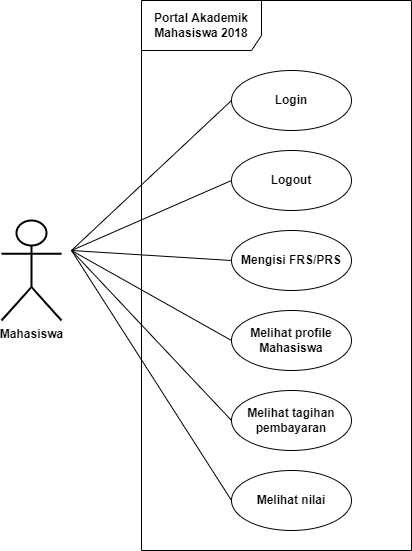
\includegraphics[scale=0.6]{Gambar/usecase.png}
	\caption{Diagram Use Case Portal Akademik Mahasiswa 2018} 
	\label{fig:usecase2018}
\end{figure}
Setelah penggambaran \textit{use case} diagram perlu dijelaskan skenario dari \textit{use case} diagram tersebut. Skenario use case merupakan alur jalannya proses \textit{use case} dari sisi aktor maupun sistemnya. Berikut ini merupakan skenario \textit{use case} yang disajikan dalam bentuk tabel.
 
\begin{figure}[H]
	\centering
	
\includegraphics[scale=0.4]{Gambar/halaman2018.jpg}
	\caption{Tampilan halaman awal Portal Akademik Mahasiswa} 
	\label{fig:studpor_home_2018}
\end{figure}
\newpage
Pada Gambar \ref{fig:studpor_home_2018} adalah tampilan awal ketika masuk ke halaman \url{https://studentportal.unpar.ac.id/}. Fitur-fitur yang tersedia pada Portal Akademik Mahasiswa sebagai berikut:
\begin{enumerate}
	\item \textit{Login}: Untuk dapat menggunakan situs Portal Akademik Mahasiswa, mahasiswa UNPAR harus \textit{login} menggunakan \textit{email} dan \textit{password} milik mahasiswa tersebut.
	\begin{itemize}
		\item Nama Use Case: \textit{Login}
		\item Aktor: Mahasiswa
		\item Deskripsi: \textit{Login} ke Portal Akademik Mahasiswa.
		\item Kondisi awal: Mahasiswa belum \textit{login}.
		\item Kondisi akhir: Halaman utama Portal Akademik Mahasiswa.
		\item Skenario utama:
		\begin{table}[h!]
			\centering
			\label{}
			\begin{tabular}{ | m{0.5cm} | m{7cm}| m{6cm} | } 
				\hline
				No & Aksi Aktor & Reaksi Sistem \\ 
				\hline
				1 & Mahasiswa mengakses Portal Akademik Mahasiswa dan menekan tombol ``Login'' & Sistem menampilkan halaman \textit{login}.
				\\ 
				\hline
				2 & Mahasiswa mengisi \textit{email} dan menekan tombol ``Next'' & Sistem menampilkan halaman \textit{input password}.
				\\ 
				\hline
				3 & Mahasiswa mengisi \textit{password} dan menekan tombol ``LOGIN'' & Sistem menampilkan halaman utama Portal Akademik Mahasiswa.
				\\ 
				\hline
			\end{tabular}
		\end{table}
	
		\begin{figure}[H] 
			\centering
			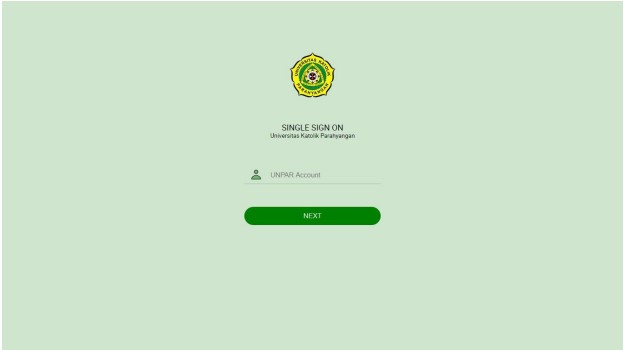
\includegraphics[scale=0.6]{Gambar/sso2018.jpg}
			\caption{Tampilan halaman untuk memasukan \textit{email} Portal Akademik Mahasiswa} 
			\label{fig:sso_2018}
		\end{figure}
		
		\begin{figure}[H] 
			\centering
			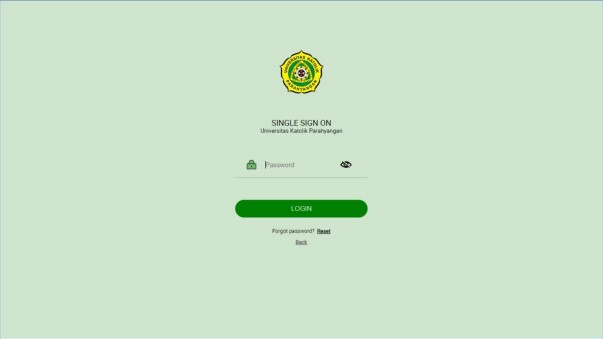
\includegraphics[scale=0.6]{Gambar/pass2018.jpg}
			\caption{Tampilan halaman untuk memasukan \textit{password} Portal Akademik Mahasiswa} 
			\label{fig:pass_2018}
		\end{figure}
		
		\begin{figure}[H]
			\centering
			
\includegraphics[scale=0.7]{Gambar/frs2018.jpg}
			\caption{Tampilan halaman utama} 
			\label{fig:frs_2018}
		\end{figure}
	\end{itemize}

	\item Fitur FRS/PRS: Untuk mengisi form rencana semester (FRS) atau melakukan perubahan rencana studi (PRS) secara online. 
	\begin{itemize}
		\item Nama Use Case: FRS/PRS
		\item Aktor: Mahasiswa
		\item Deskripsi: Melakukan FRS/PRS Portal Akademik Mahasiswa.
		\item Kondisi awal: Mahasiswa telah \textit{login}.
		\item Kondisi akhir: Halaman FRS/PRS pada Portal Akademik Mahasiswa.
		\item Skenario utama:
		\begin{table}[h!]
			\centering
			\label{}
			\begin{tabular}{ | m{0.5cm} | m{7cm}| m{6cm} | } 
				\hline
				No & Aksi Aktor & Reaksi Sistem \\ 
				\hline
				1 & Mahasiswa memilih menu ``FRS/PRS'' & Sistem menampilkan halaman FRS/PRS.
				\\ 
				\hline
			\end{tabular}
		\end{table}	
	\end{itemize}

	\item Fitur Profil Mahasiswa: Untuk melihat profil milik mahasiswa itu sendiri.
	\begin{itemize}
		\item Nama Use Case: Profil
		\item Aktor: Mahasiswa
		\item Deskripsi: Melihat data diri mahasiswa pada Portal Akademik Mahasiswa.
		\item Kondisi awal: Mahasiswa telah \textit{login}.
		\item Kondisi akhir: Halaman Profil pada Portal Akademik Mahasiswa.
		\item Skenario utama:
		\begin{table}[h!]
			\centering
			\label{}
			\begin{tabular}{ | m{0.5cm} | m{7cm}| m{6cm} | } 
				\hline
				No & Aksi Aktor & Reaksi Sistem \\ 
				\hline
				1 & Mahasiswa memilih menu Profil & Sistem menampilkan halaman Profil.
				\\ 
				\hline
			\end{tabular}
		\end{table}	
	\end{itemize}
	\begin{figure}[H]
		\centering
		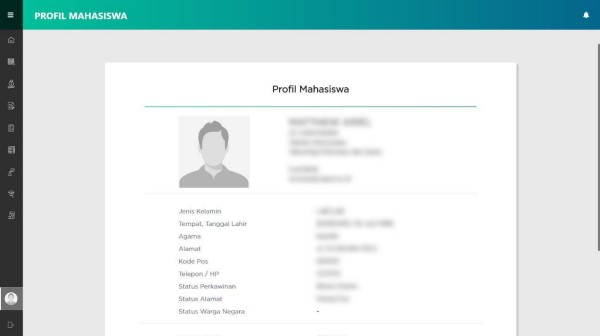
\includegraphics[scale=0.7]{Gambar/profil2018.jpg}
		\caption{Tampilan halaman profil mahasiswa} 
		\label{fig:profil_2018}
	\end{figure}

	
	\item Fitur Pembayaran: Menampilkan jenis tagihan dan jumlah tagihan dari setiap jenis tagihan yang ada.
	\begin{itemize}
		\item Nama Use Case: Pembayaran
		\item Aktor: Mahasiswa
		\item Deskripsi: Melihat jenis tagihan dan jumlah tagihan pembayaran semester milik mahasiswa pada Portal Akademik Mahasiswa.
		\item Kondisi awal: Mahasiswa telah \textit{login}
		\item Kondisi akhir: Halaman pembayaran pada Portal Akademik Mahasiswa.
		\item Skenario utama:
		\begin{table}[h!]
			\centering
			\label{}
			\begin{tabular}{ | m{0.5cm} | m{7cm}| m{6cm} | } 
				\hline
				No & Aksi Aktor & Reaksi Sistem \\ 
				\hline
				1 & Mahasiswa memilih menu Pembayaran & Sistem menampilkan halaman Pembayaran.
				\\ 
				\hline
			\end{tabular}
		\end{table}	
	\end{itemize}
	\begin{figure}[H]
		\centering
		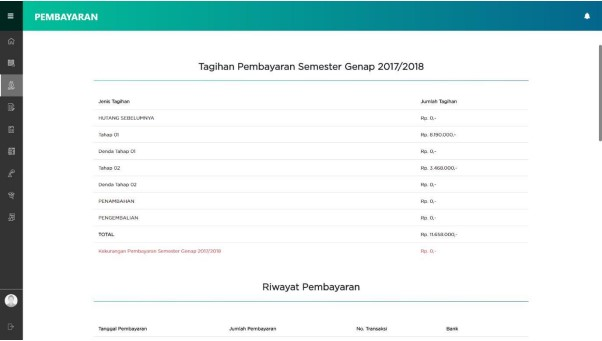
\includegraphics[scale=0.7]{Gambar/bayar2018.jpg}
		\caption{Tampilan halaman pembayaran bagian Tagihan Pembayaran} 
		\label{fig:bayar_2018}
	\end{figure}
	\begin{figure}[H]
		\centering
		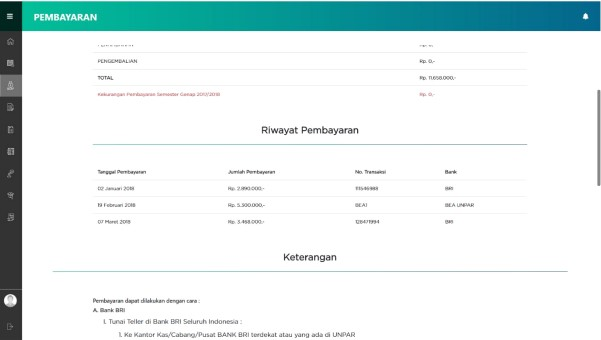
\includegraphics[scale=0.7]{Gambar/riwayat2018.jpg}
		\caption{Tampilan halaman pembayaran bagian Riwayat Pembayaran} 
		\label{fig:riw_2018}
	\end{figure}
	\begin{figure}[H]
		\centering
		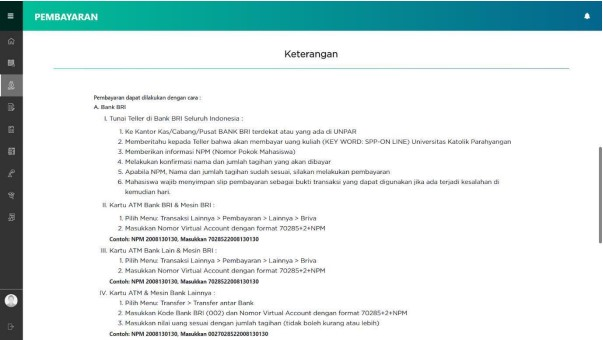
\includegraphics[scale=0.7]{Gambar/keterangan2018.jpg}
		\caption{Tampilan halaman pembayaran bagian Keterangan} 
		\label{fig:ketbayar_2018}
	\end{figure}

	\item Fitur Nilai: Melihat semua nilai milik mahasiswa dari setiap semester.
	\begin{itemize}
		\item Nama Use Case: Nilai
		\item Aktor: Mahasiswa
		\item Deskripsi: Melihat nilai milik mahasiswa.
		\item Kondisi awal: Mahasiswa telah \textit{login}
		\item Kondisi akhir: Halaman nilai mahasiswa pada Portal Akademik Mahasiswa.
		\item Skenario utama:
		\begin{table}[h!]
			\centering
			\label{}
			\begin{tabular}{ | m{0.5cm} | m{7cm}| m{6cm} | } 
				\hline
				No & Aksi Aktor & Reaksi Sistem \\ 
				\hline
				1 & Mahasiswa memilih menu Nilai & Sistem menampilkan halaman Nilai per semester.
				\\ 
				\hline
				2 & Mahasiswa memilih menu Riwayat Index Prestasi & Sistem menampilkan halaman Riwayat Index Prestasi.
				\\ 
				\hline
			\end{tabular}
		\end{table}	
	\end{itemize}
	\begin{figure}[H]
		\centering
		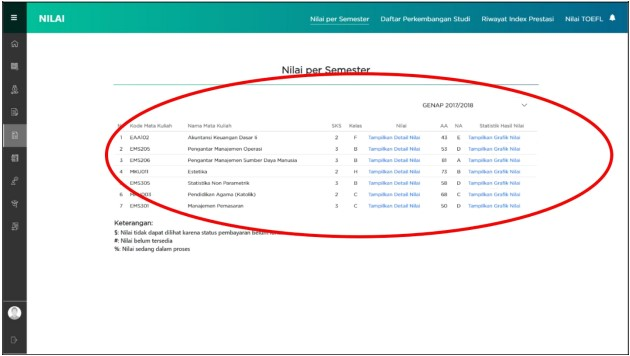
\includegraphics[scale=0.7]{Gambar/nilai2018.jpg}
		\caption{Tampilan halaman nilai bagian Nilai per Semester} 
		\label{fig:nilai_2018}
	\end{figure}
	\begin{figure}[H]
		\centering
		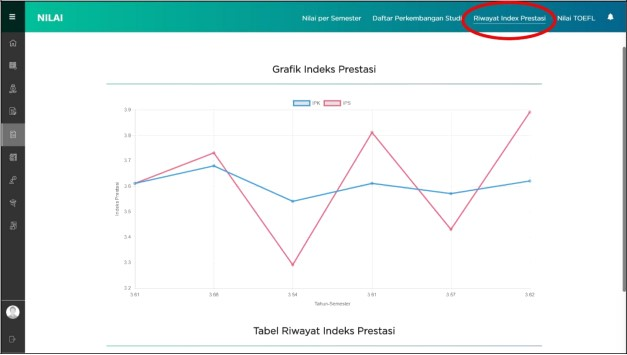
\includegraphics[scale=0.7]{Gambar/rip2018.jpg}
		\caption{Tampilan halaman nilai bagian Riwayat Index Prestasi} 
		\label{fig:rip_2018}
	\end{figure}
\end{enumerate}
Portal Akademik Mahasiswa 2018 belum memiliki fitur perekaman kehadiran secara daring. Hal tersebut dikarenakan belum adanya pembelajaran secara daring, sehingga perekaman kehadiran dilakukan secara luring yang dimana perekaman kehadiran dilakukan secara langsung saat pembelajaran tatap muka.

\subsection{Fitur Tambahan Perekaman Kehadiran Portal Akademik Mahasiswa}
\label{sec:alur} 
Portal Akademik Mahasiswa Universitas Katolik Parahyangan yang terbaru sejak 2020 sudah memiliki fitur perekaman kehadiran daring. Fitur tersebut dapat melakukan perekaman kehadiran secara daring untuk setiap mata kuliah yang diambil. Diagram \textit{use case} dilihat di Gambar \ref{fig:usecase2020}.

\begin{figure}[H]
	\centering
	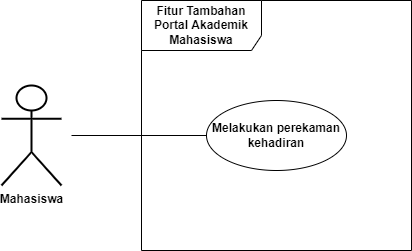
\includegraphics[scale=0.6]{Gambar/usecase2020.png}
	\caption{Diagram Use Case Fitur Tambahan Portal Akademik Mahasiswa} 
	\label{fig:usecase2020}
\end{figure}
Skenario \textit{use case} ini merupakan tambahan lanjutan fitur dari use case pada subbab \ref{sec:pam} yang tidak memiliki fitur perekaman kehadiran daring. 
\begin{itemize}
	\item Nama Use Case: Jadwal \& Kehadiran
	\item Aktor: Mahasiswa
	\item Deskripsi: Melihat jadwal mata kuliah dan melakukan absensi daring pada Portal Akademik Mahasiswa. 
	\item Kondisi awal: Mahasiswa telah \textit{login}
	\item Kondisi akhir: Halaman Jadwal \& Kehadiran dan mahasiswa berhasil melakukan absensi daring.
	\item Skenario utama:
	\begin{table}[h!]
		\centering
		\label{}
		\begin{tabular}{ | m{0.5cm} | m{7cm}| m{6cm} | } 
			\hline
			No & Aksi Aktor & Reaksi Sistem \\ 
			\hline
			1 & Mahasiswa memilih menu Jadwal \& Kehadiran & Sistem menampilkan halaman Jadwal \& Kehadiran per-semester (Gambar \ref{fig:absen}).
			\\ 
			\hline
			2 & Mahasiswa menekan tombol berwarna merah pada kolom presensi pada tabel jadwal kehadiran & Sistem menampilkan notifikasi mengenai absensi berhasil dilakukan (Gambar\ref{fig:berhasil}).
			\\ 
			\hline
			3 & Mahasiswa menekan tombol ``OK'' & Sistem menutup notifikasi.
			\\ 
			\hline
		\end{tabular}
	\end{table}	
\end{itemize}
Diagram aktivitas untuk perekaman kehadiran daring pada Portal Akademik Mahasiswa dapat dilihat di Gambar \ref{fig:acPAM}. Diagram aktifitas tersebut menunjukan bagaimana alur dalam melakukan perekaman kehadiran daring secara manual. Pada diagram aktivitas dapat dilihat bahwa banyak urutan langkah yang perlu dilakukan oleh mahasiswa untuk melakukan perekaman kehadiran daring. Diagram aktivitas ini untuk dapat dibandingkan perbedaannya dengan program yang akan dibuat, sehingga mengetahui langkah-langkah apa saja yang dipersingkat untuk diotomatisasi.

\begin{figure}[H]
	\centering
	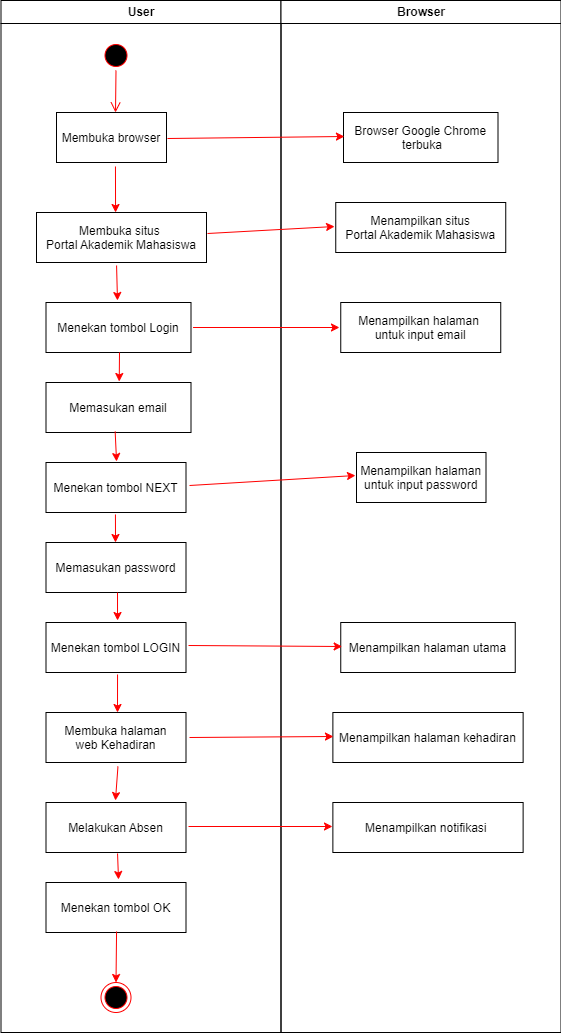
\includegraphics[scale=0.55]{Gambar/activityPAM.png}
	\caption{Diagram Aktivitas Portal Akademik Mahasiswa 2020} 
	\label{fig:acPAM}
\end{figure}

Setiap mahasiswa sebelum memulai perkuliahan pada setiap mata kuliah perlu mengakses Portal Akademik Mahasiswa yang dapat diakses melalui \url{https://studentportal.unpar.ac.id/} seperti pada Gambar \ref{fig:studpor_home_2019}. 
\begin{figure}[H]
	\centering
	
\includegraphics[scale=0.225]{Gambar/halaman2019.jpg}
	\caption{Tampilan halaman awal Portal Akademik Mahasiswa} 
	\label{fig:studpor_home_2019}
\end{figure}

Setelah itu mahasiswa melakukan \textit{Login} dengan mengisi \textit{email} serta \textit{password} milik mahasiswa tersebut. Pada Gambar \ref{fig:login} merupakan tampilan untuk mengisi \textit{email} dan Gambar \ref{fig:pass} merupakan tampilan untuk mengisi \textit{password}.
\begin{figure}[H]
	\centering
	
\includegraphics[scale=0.225]{Gambar/login.jpg}
	\caption{Tampilan halaman Portal Akademik Mahasiswa untuk memasukan \textit{email}} 
	\label{fig:login}
\end{figure}

\begin{figure}[H]
	\centering
	
\includegraphics[scale=0.225]{Gambar/pass.jpg}
	\caption{Tampilan halaman Portal Akademik Mahasiswa untuk memasukan \textit{password}} 
	\label{fig:pass}
\end{figure}
\newpage
Setelah berhasil melakukan \textit{login} akan ada dua kemungkinan yang terjadi pada halaman Portal Akademik Mahasiswa, yaitu pertama akan muncul notifkasi peringatan seperti pada Gambar \ref{fig:notif} dan kedua akan masuk langsung ke halaman utama Portal Akademik Mahasiswa seperti pada Gambar \ref{fig:jadwal}. Jika muncul notifikasi terlebih dahulu maka harus menutup notifikasi tersebut untuk dapat masuk ke halaman utama.
\begin{figure}[H]
	\centering
	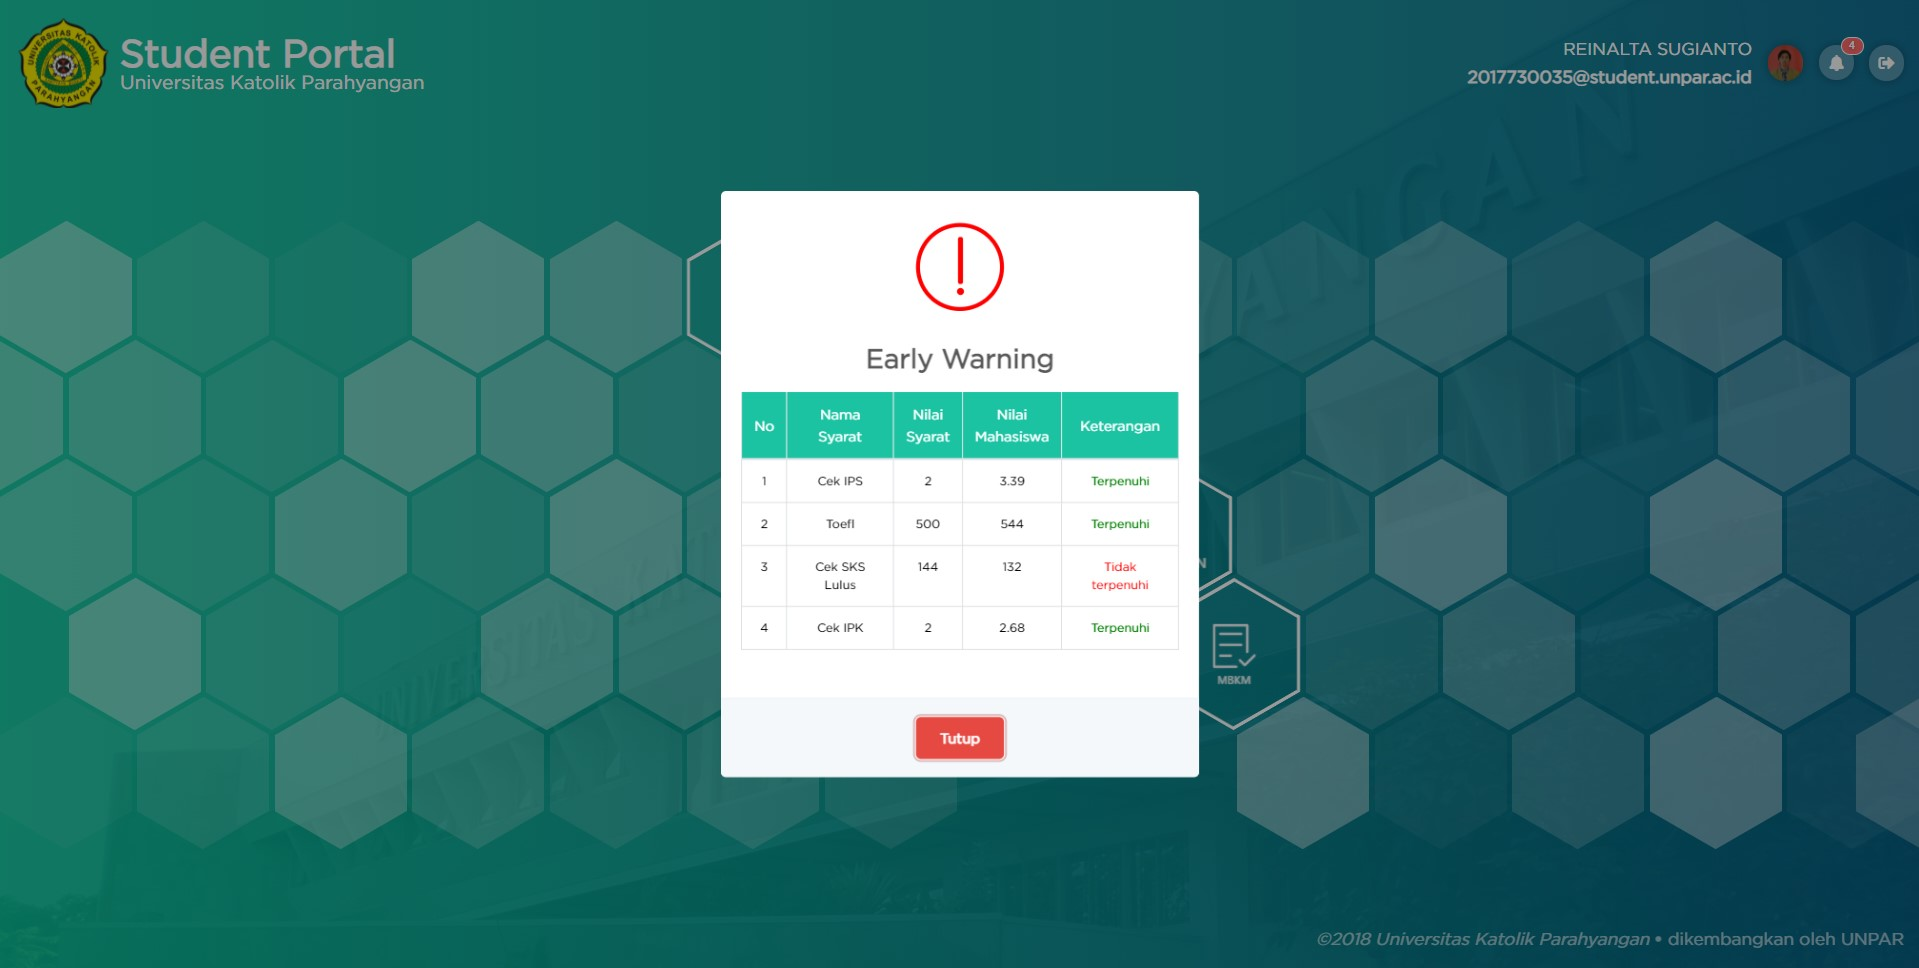
\includegraphics[scale=0.225]{Gambar/notif.jpg}
	\caption{Tampilan peringatan pada halaman Portal Akademik Mahasiswa} 
	\label{fig:notif}
\end{figure}

\begin{figure}[H]
	\centering
	
\includegraphics[scale=0.225]{Gambar/jadwal.jpg}
	\caption{Tampilan halaman Portal Akademik Mahasiswa setelah Berhasil \textit{Login}} 
	\label{fig:jadwal}
\end{figure}

Pada Gambar \ref{fig:notif} merupakan sebuah peringatan yang terkadang muncul menjelang berakhirnya suatu semester untuk melihat status kebutuhan mahasiswa untuk lulus, sehingga perlu menekan tombol ``Tutup'' terlebih dahulu untuk menekan tombol berbentuk heksagon ``JADWAL \& KEHADIRAN'' seperti pada Gambar \ref{fig:jadwal}. Jika tidak terjadi peringatan seperti pada  Gambar \ref{fig:notif}, maka dapat langsung menekan tombol berbentuk heksagon ``JADWAL \& KEHADIRAN'' seperti pada Gambar \ref{fig:jadwal}.

Setelah berhasil masuk ke halaman untuk perekaman kehadiran daring, mahasiswa perlu menekan tombol berwarna merah pada kolom bagian presensi pada tabel jadwal kehadiran mata kuliah (Gambar \ref{fig:absen}). Setelah mengklik tombol presensi maka akan muncul notifikasi bahwa absensi telah berhasil dan mahasiswa perlu menekan tombol ``OK''. 	
\begin{figure}[H]
	\centering
	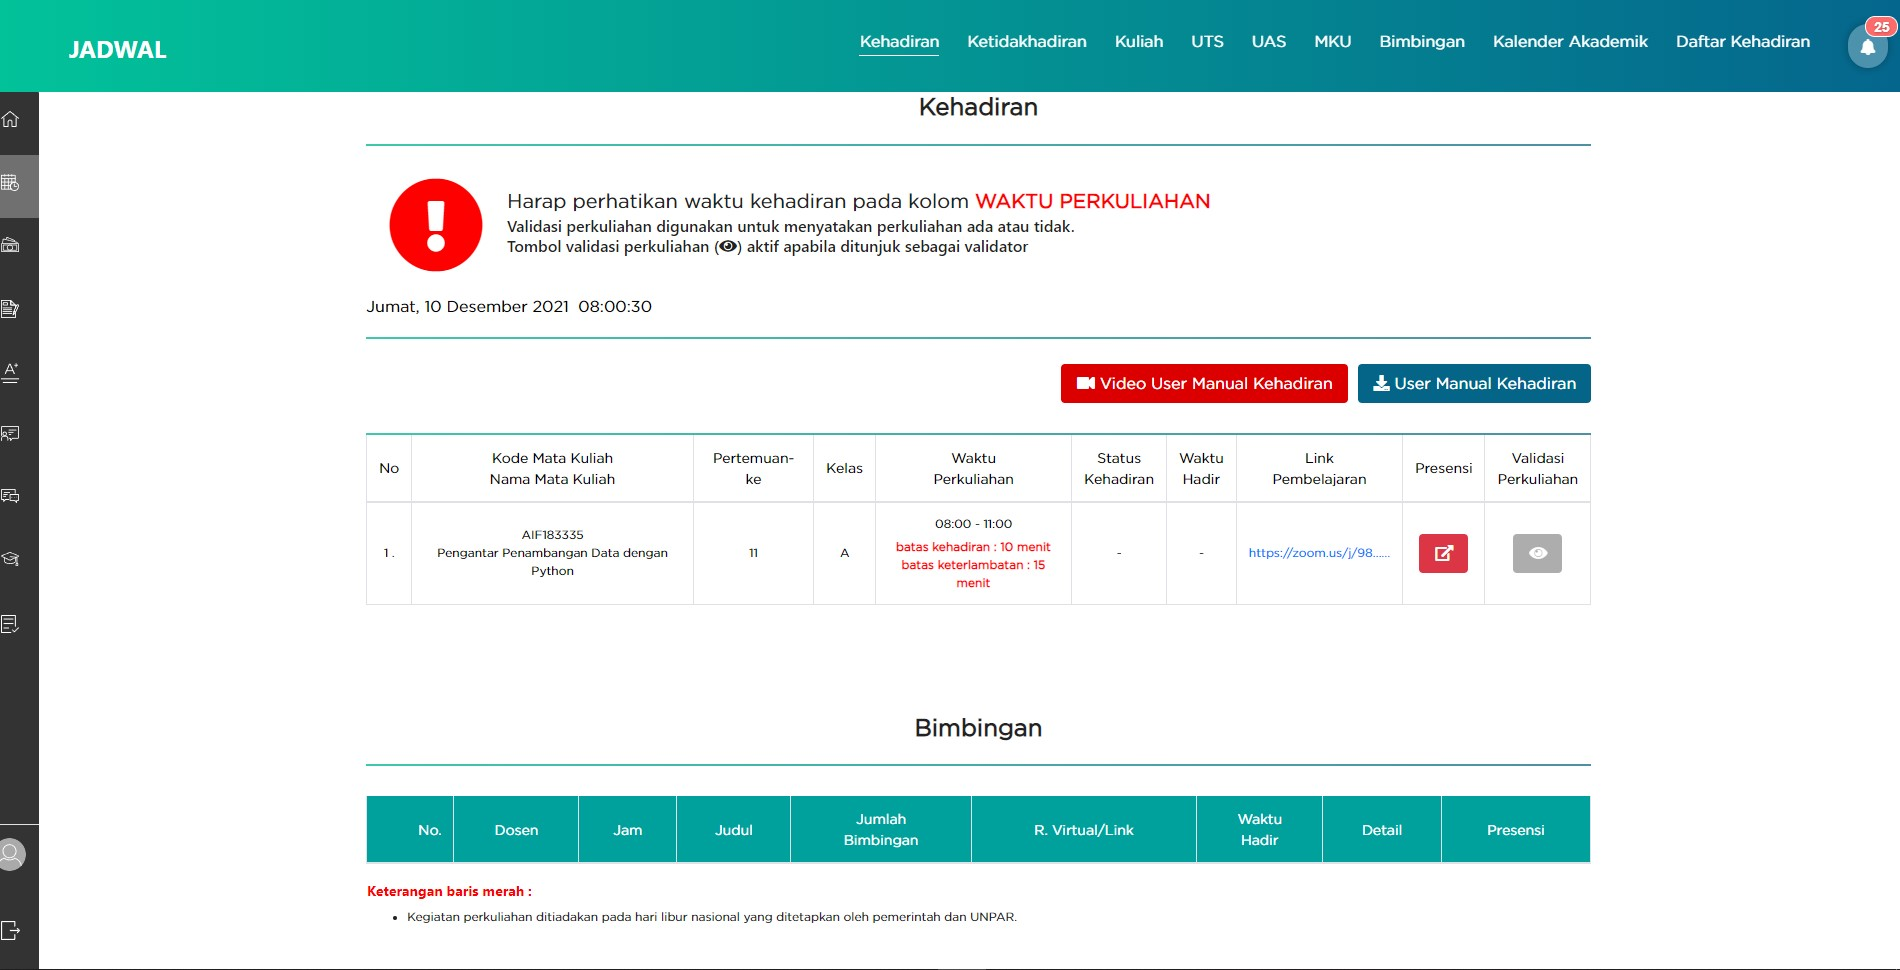
\includegraphics[scale=0.225]{Gambar/absen.jpg}
	\caption{Tampilan halaman Portal Akademik Mahasiswa untuk Melakukan Absen} 
	\label{fig:absen}
\end{figure}
\begin{figure}[H]
	\centering
	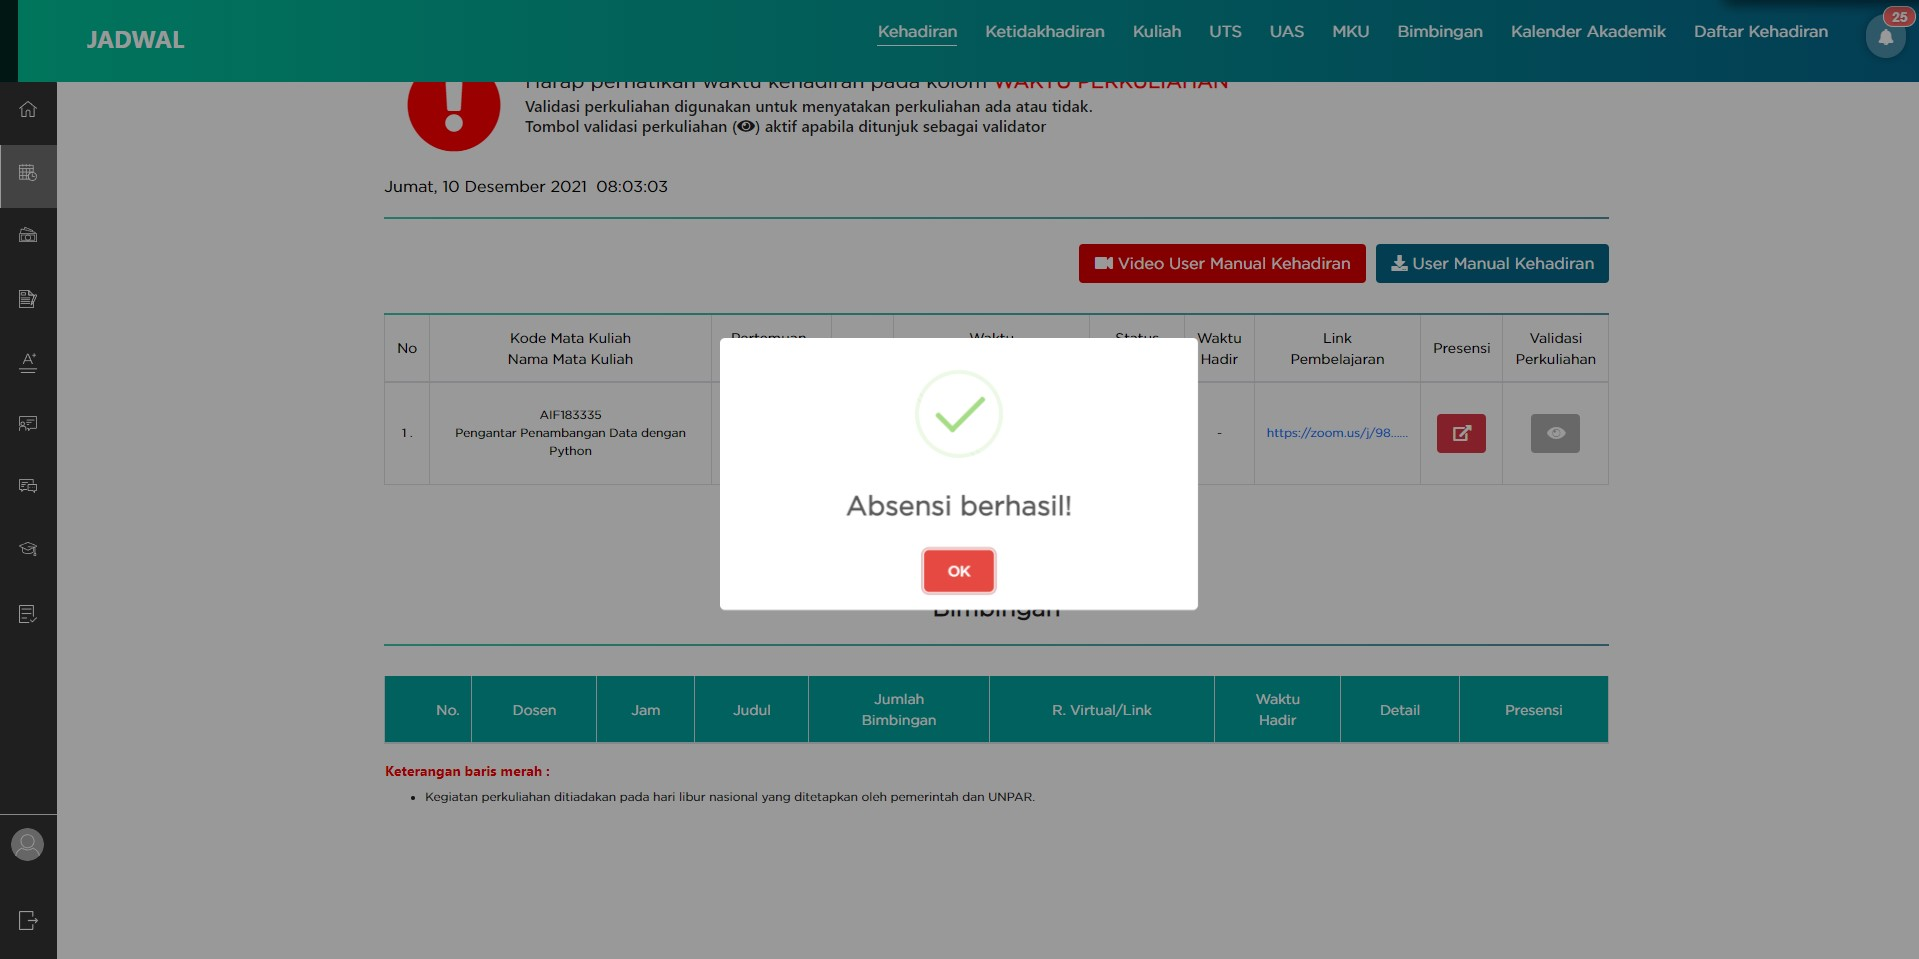
\includegraphics[scale=0.225]{Gambar/berhasilAbsen.jpg}
	\caption{Tampilan Pemberitahuan Absensi Berhasil} 
	\label{fig:berhasil}
\end{figure}

\subsection{AKUHADIR 2.1}\vspace{-0.2cm}
\label{sec:akuhadir}
Subbab ini ditulis dari hasil mewawancarai dosen pembimbing, karena penulis tidak memiliki akses terhadap AKUHADIR. AKUHADIR adalah sebuah portal web yang dibuat bagi pegawai UNPAR dalam melaporkan kehadiran kerja nya secara daring. Pegawai UNPAR melakukan perekaman kehadirannya setiap hari melalui portal AKUHADIR 2.1 yang dapat diakses pada \url{https://akuhadir.unpar.ac.id}. Hal tersebut sesuai surat edaran dari Rektor III/R/2020-07/1153 \cite{akuhadir}. Diagram \textit{use case} dapat dilihat pada Gambar \ref{fig:usecaseDosen}.
\begin{figure}[H] \vspace{-0.35cm}
	\centering
	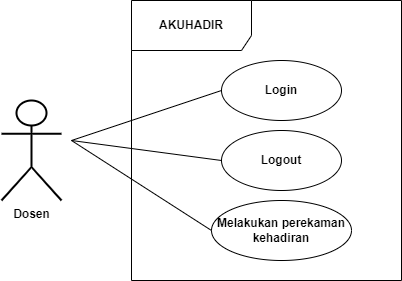
\includegraphics[scale=0.5]{Gambar/usecaseDosen.png}
	\caption{Diagram Use Case AKUHADIR} 
	\label{fig:usecaseDosen}
\end{figure}

Setelah penggambaran \textit{use case} diagram perlu dijelaskan skenario dari \textit{use case} diagram tersebut. Skenario use case merupakan alur jalannya proses \textit{use case} dari sisi aktor maupun sistemnya. Berikut ini merupakan skenario \textit{use case} yang disajikan dalam bentuk tabel.

\begin{enumerate}
	\item Fitur \textit{Login}: Untuk dapat menggunakan situs AKUHADIR, dosen UNPAR harus \textit{login} menggunakan \textit{email} dan \textit{password} milik dosen tersebut.
	\begin{itemize}
		\item Nama Use Case: \textit{Login}
		\item Aktor: Dosen
		\item Deskripsi: \textit{Login} ke situs AKUHADIR.
		\item Kondisi awal: Dosen belum \textit{login}.
		\item Kondisi akhir: Halaman utama AKUHADIR.
		\item Skenario utama:
		\begin{table}[h!]
			\centering
			\label{}
			\begin{tabular}{ | m{0.5cm} | m{7cm}| m{6cm} | } 
				\hline
				No & Aksi Aktor & Reaksi Sistem \\ 
				\hline
				1 & Dosen mengakses AKUHADIR  & Sistem menampilkan halaman \textit{login}.
				\\ 
				\hline
				2 & Dosen mengisi \textit{email} dan menekan tombol ``Next'' & Sistem menampilkan halaman \textit{input password}.
				\\ 
				\hline
				3 & Dosen mengisi \textit{password} dan menekan tombol ``LOGIN'' & Sistem menampilkan halaman utama AKUHADIR.
				\\ 
				\hline
			\end{tabular}
		\end{table}
	\end{itemize}
	\item Fitur WFH: Melakukan absen daring bagi dosen pada situs AKUHADIR.
	\begin{itemize}
		\item Nama Use Case: \textit{WFH}
		\item Aktor: Dosen
		\item Deskripsi: Melakukan absensi daring pada situs AKUHADIR.
		\item Kondisi awal: Dosen telah \textit{login}.
		\item Kondisi akhir: Halaman WFH dan dosen berhasil melakukan absensi daring.
		\item Skenario utama:
		\begin{table}[h!]
			\centering
			\label{}
			\begin{tabular}{ | m{0.5cm} | m{7cm}| m{6cm} | } 
				\hline
				No & Aksi Aktor & Reaksi Sistem \\ 
				\hline
				1 & Dosen memilih menu WFH  & Sistem menampilkan halaman WFH.
				\\ 
				\hline
				2 & Dosen menekan tombol \textit{CHECK IN} & Sistem menampilkan pesan konfirmasi bahwa absensi dosen berhasil.
				\\ 
				\hline
			\end{tabular}
		\end{table}	
	\end{itemize}
\end{enumerate}

Gambar \ref{fig:akuhadir-1-beranda} menunjukkan halaman awal portal AKUHADIR. Pegawai UNPAR melakukan \textit{login} melalui SSO (\textit{Single Sign On}) UNPAR untuk dapat melakukan perekaman kehadirannya. Setelah melakukan login para pegawai UNPAR dapat melakukan perekaman kehadiran secara daring dengan memilih menu WFH pada bagian bawah layar. Menu WFH ini akan membuka halaman di mana pegawai UNPAR dapat melakukan perekaman kehadiran. Halaman tersebut terdapat dua buah tombol, yaitu: satu tombol untuk \textit{check in} dan satu tombol lagi untuk \textit{check out}. Halaman dari menu WFH dapat dilihat pada Gambar \ref{fig:akuhadir-2-wfh}.
\begin{figure}[H]
	\centering
	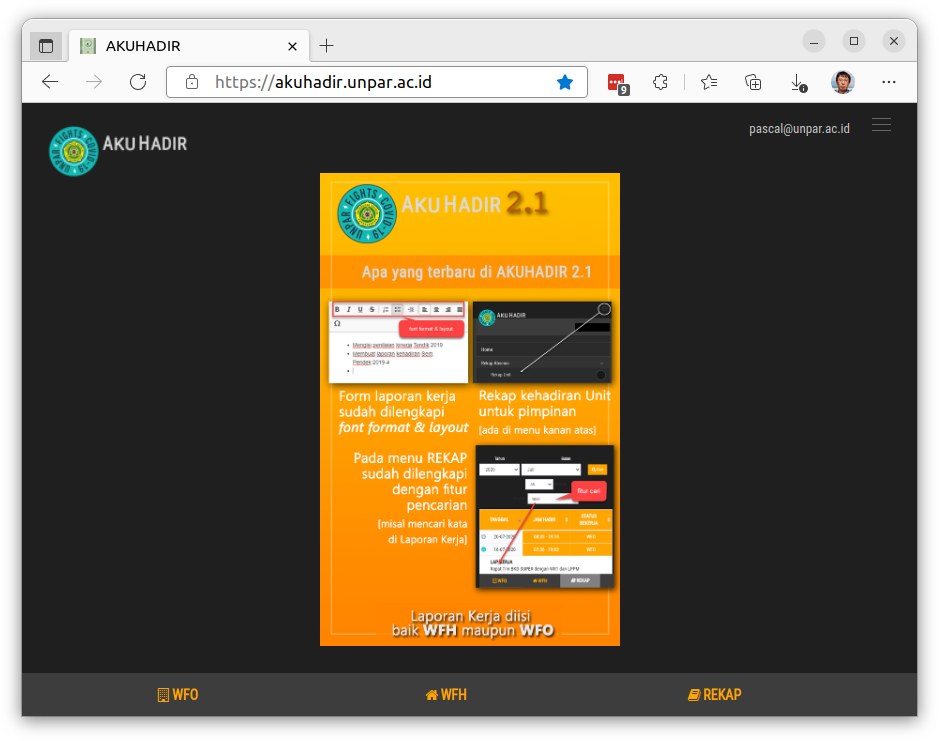
\includegraphics[scale=0.3]{Gambar/akuhadir-1-beranda.png}
	\caption{Tampilan awal halaman AKUHADIR} 
	\label{fig:akuhadir-1-beranda}
\end{figure}

Pegawai UNPAR sebelum memulai bekerja di pagi hari harus melakukan perekaman kehadiran melalui AKUHADIR. Pegawai membuka situs AKUHADIR dan \textit{login} sesuai dengan \textit{email} serta \textit{password} milik pegawai. Pegawai mengklik menu WFH untuk masuk ke bagian halaman perekaman kehadiran milik situs AKUHADIR. Selanjutnya pegawai mengklik menu \textit{Check in}. Setelah tombol tersebut diklik, akan muncul pesan konfirmasi bahwa \textit{check in} sudah berhasil dilakukan (dapat dilihat pada Gambar \ref{fig:akuhadir-3-wfh-checkin}).

\begin{figure}[H]
	\centering
	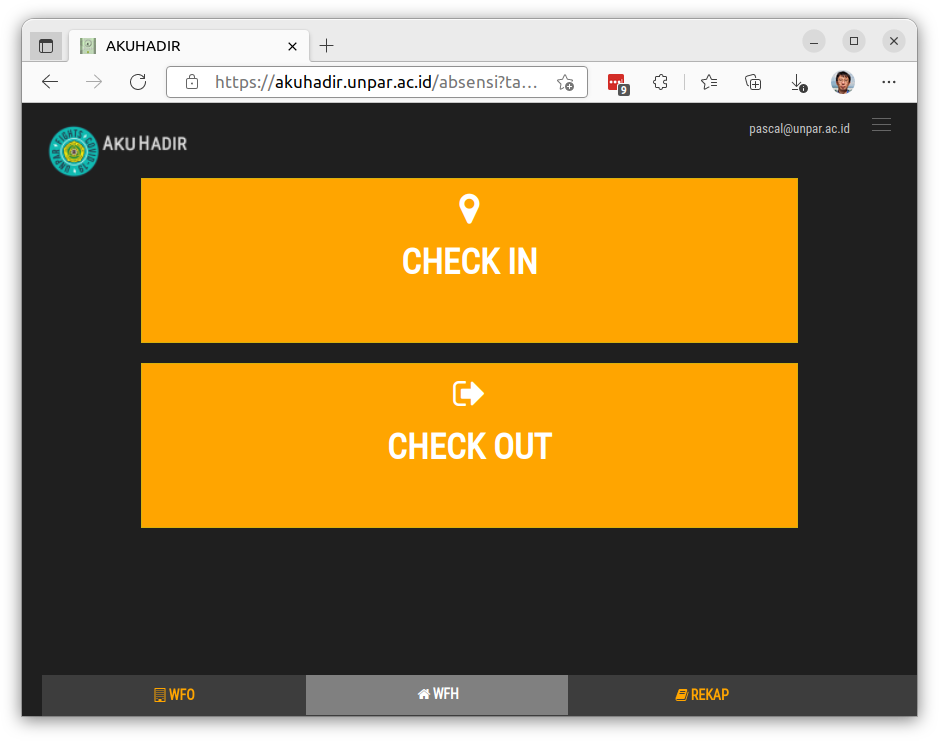
\includegraphics[scale=0.3]{Gambar/akuhadir-2-wfh.png}
	\caption{Tampilan menu WFH} 
	\label{fig:akuhadir-2-wfh}
\end{figure}

\begin{figure}[H]
	\centering
	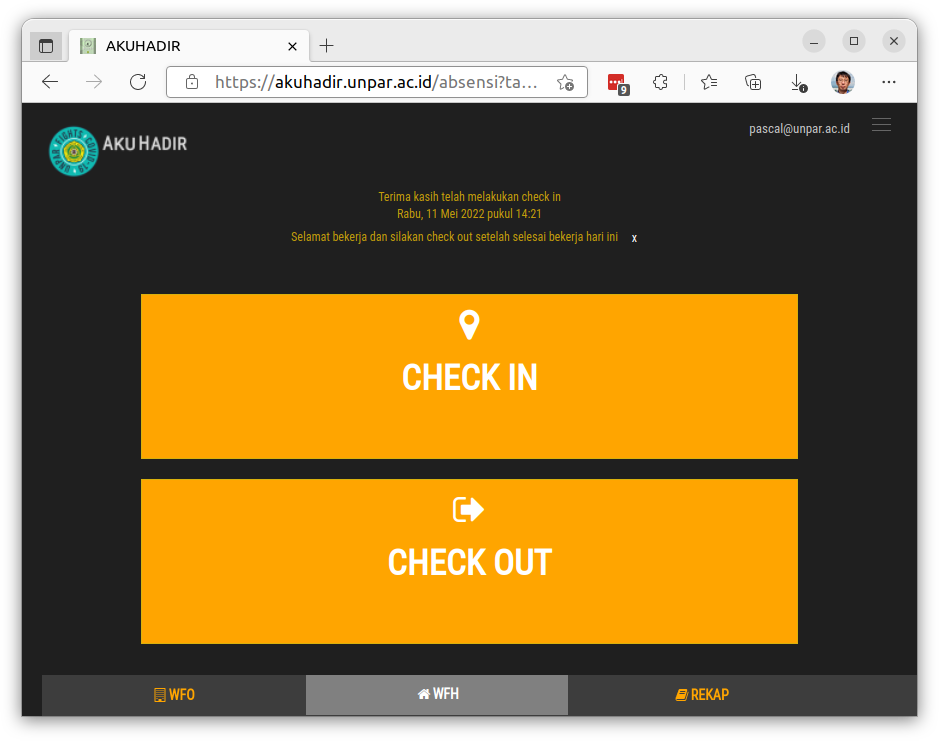
\includegraphics[scale=0.3]{Gambar/akuhadir-3-wfh-checkin.png}
	\caption{Tampilan konfirmasi check in AKUHADIR} 
	\label{fig:akuhadir-3-wfh-checkin}
\end{figure}

Setelah selesai bekerja, pegawai perlu kembali mengakses AKUHADIR dan masuk ke halaman perekaman kehadiran dari menu WFH. Lalu pegawai memilih menu \textit{check out}. Setelah melakukan \textit{check out}, pegawai UNPAR diminta untuk menuliskan laporan hasil pekerjaan yang sudah dilakukan pada hari tersebut. Bentuk halaman untuk menuliskan laporan hasil pekerjaan pada Gambar \ref{fig:akuhadir-4-wfh-checkout}.

\begin{figure}[H]
	\centering
	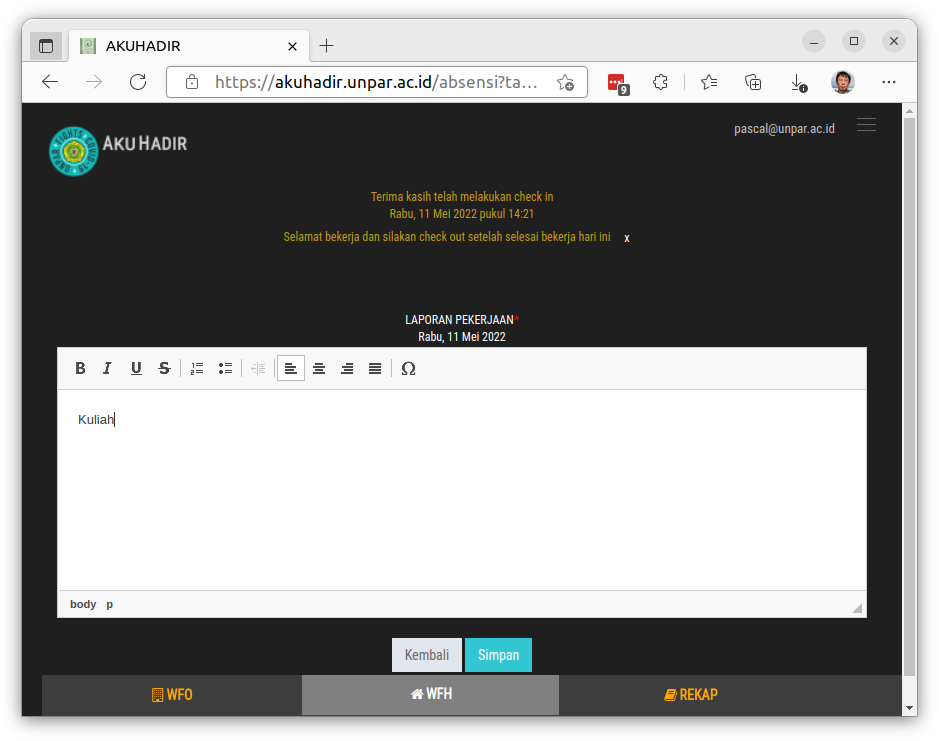
\includegraphics[scale=0.3]{Gambar/akuhadir-4-wfh-checkout.png}
	\caption{Tampilan halaman check out AKUHADIR} 
	\label{fig:akuhadir-4-wfh-checkout}
\end{figure}
Selain fitur untuk melakukan perekaman kehadiran daring pada AKUHADIR, terdapat beberapa fitur lainnya yang tidak dijelaskan lebih mendalam di sini karena tidak terkait erat dengan penelitian yang dilakukan:

\begin{itemize}
	\item \textbf{WFO} untuk melihat status pelaporan bekerja dari kantor (pelaporan bekerja dari kantor dilakukan oleh petugas keamanan UNPAR yang memindai kode batang pegawai).
	\item \textbf{Rekap} untuk melihat rekapitulasi pelaporan bekerja, baik WFH maupun WFO.
	\item \textbf{Profil} untuk menampilkan foto serta kode batang pegawai. Bisa digunakan untuk menunjukkan kode batang kepada petugas keamanan dalam rangka pelaporan WFO.
	\item \textbf{About} saat ini hanya menampilkan informasi versi dan \textit{copyright}.
\end{itemize}

\section{Analisis Sistem Sejenis}

\subsection{Selenium IDE}
\label{sec:seleniumIDE}  
Selenium IDE merupakan program \textit{open source} untuk otomatisasi di web. Selenium IDE dapat di \textit{install} di browser, contohnya di Google Chrome yang setelah di \textit{install} akan menjadi \textit{extensions}. \textit{Extensions} di Google Chrome adalah sebuah aplikasi kecil yang dapat dijalankan pada Google Chrome itu sendiri. Berikut ini cara untuk melakukan otomatisasi menggunakan Selenium IDE:
\begin{enumerate}
	\item Membuka Selenium Ide yang tersimpan di \textit{Extensions} pada Google Chrome.
	\item Memilih menu \textit{Record a new test in a new project} (merekam tes baru untuk proyek baru).
	\begin{figure}[H]
		\centering
		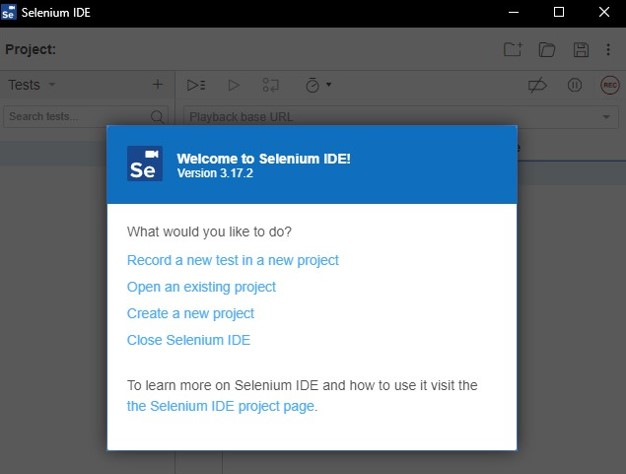
\includegraphics[scale=0.5]{Gambar/menuSeleniumIDE.jpg}
		\caption{Tampilan Menu Awal Selenium IDE} 
		\label{fig:menuSeleniumIDE}
	\end{figure}
	\newpage
	\item Memasukan nama proyek, lalu tekan tombol ``OK''. 
	\begin{figure}[H]
		\centering
		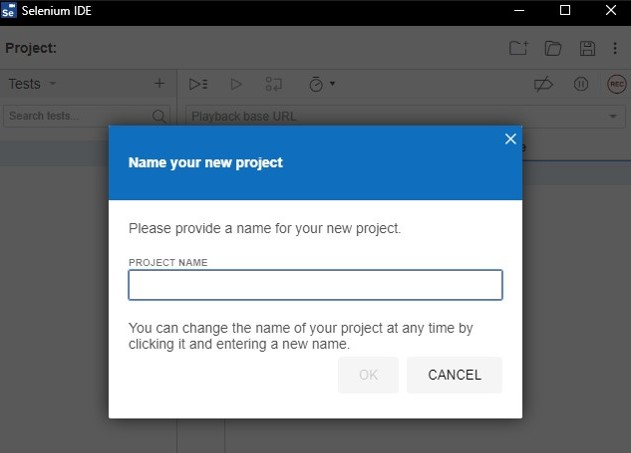
\includegraphics[scale=0.4]{Gambar/namaProyek.jpg}
		\caption{Tampilan Memasukan Nama Proyek} 
		\label{fig:namaProyek}
	\end{figure}
	\item Memasukan situs web, lalu menekan tombol ``START RECORDING''
	\begin{figure}[H]
		\centering
		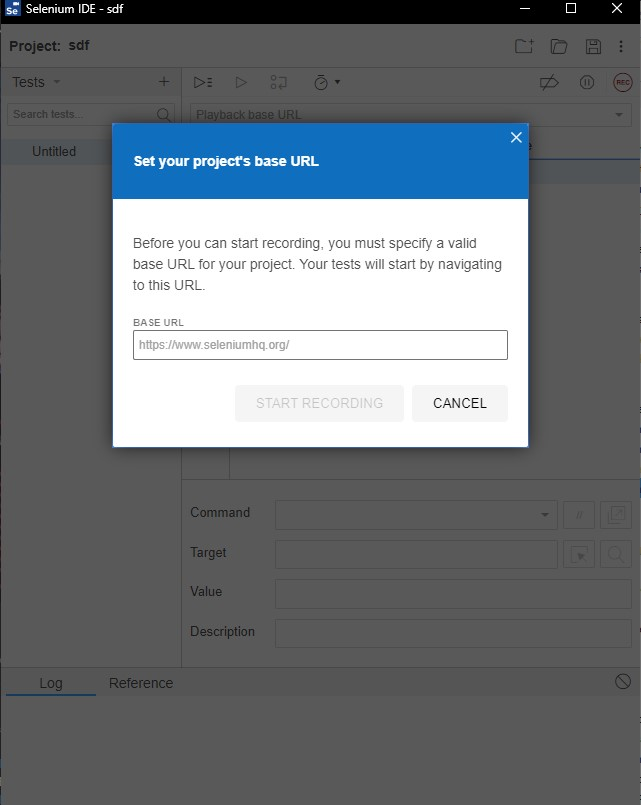
\includegraphics[scale=0.4]{Gambar/baseURL.jpg}
		\caption{Tampilan Memasukan Situs Web} 
		\label{fig:baseURL}
	\end{figure}
	Setelah menekan tombol ``\textit{START RECORDING}'' seperti pada Gambar \ref{fig:baseURL}, maka akan langsung muncul \textit{windows} Google Chrome baru yang langsung menuju situs web yang sudah dimasukan tadi.
	\item Melakukan apa yang ingin diotomatisasikan di \textit{windows} Google Chrome baru yang sudah menuju situs web hingga selesai dan menutup \textit{windows} Google Chrome. 
	Pada Gambar \ref{fig:testing} menunjukan hasil yang sudah terekam dari apa yang sudah dilakukan pada situs web yang ingin diotomatisasikan.
	\begin{figure}[H]
		\centering
		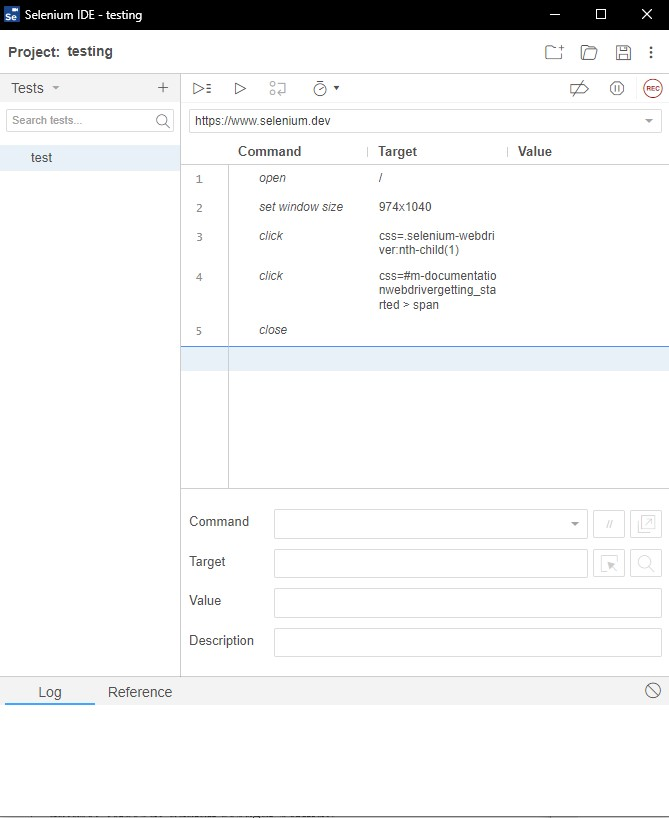
\includegraphics[scale=0.5]{Gambar/testing.jpg}
		\caption{Tampilan Otomatisasi pada Selenium IDE} 
		\label{fig:testing}
	\end{figure}	
\end{enumerate}

Selenium IDE ini dapat digunakan untuk melakukan perekaman kehadiran otomatis pada Portal Akademik Mahasiswa. Program yang dibuat pada skripsi ini akan sejenis dengan Selenium IDE, namun program pada skripsi ini akan dapat dijalankan langsung melalui \textit{Command Prompt}. Pada program yang dibuat di skripsi ini membuat pengguna tidak perlu melakukan seperti pada Selenium IDE. Pengguna cukup menjalankan melalui \textit{Command Prompt} saja.

\section{Analisis Sistem Usulan}

\subsection{Analisis Hasil Survei Perekaman Kehadiran Daring dan Luring}
\label{sec:survei} 
Survei perekaman kehadiran daring dan luring dilakukan untuk mengetahui berapa lama waktu yang dibutuhkan untuk melakukan perekaman kehadiran secara daring maupun luring dan beberapa informasi dalam melakukan perekaman kehadiran daring. Survei ini diberikan kepada mahasiswa dan dosen Teknik Informatika Universitas Katolik Parahyangan. Hasil survei menunjukan bahwa waktu yang dibutuhkan untuk perekaman kehadiran secara luring lebih cepat bagi para mahasiswa maupun dosen dibandingkan waktu yang dibutuhkan untuk perekaman kehadiran secara daring.

\subsubsection{Hasil Survei Mahasiswa}
Berdasarkan hasil survei yang telah diterima dari 21 orang responden yang merupakan mahasiswa Teknik Informatika Universitas Katolik
Parahyangan yang terdiri dari mahasiswa angkatan 2017 sampai 2019, dengan pertanyaan yang diajukan kepada responen dan rangkuman jawaban hasil survei sebagai berikut:
\begin{enumerate}
	\item \textbf{Berapa detik perkiraan waktu interaksi yang Anda butuhkan untuk melakukan perekaman kehadiran daring di \url{https://studentportal.unpar.ac.id/}, mulai dari membuka \textit{browser}, lalu masuk ke \url{https://studentportal.unpar.ac.id/}, lalu mengklik tombol presensi?}
	\begin{figure}[H]
		\centering
		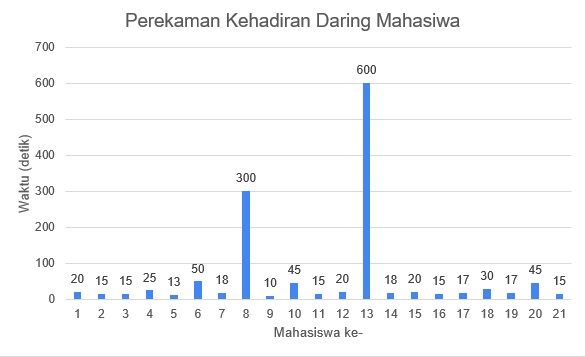
\includegraphics[scale=0.6]{Gambar/DaringMahasiswa.jpg}
		\caption{Histogram Waktu Perekaman Kehadiran Daring Mahasiswa} 
		\label{fig:DaringMahasiswa}
	\end{figure}
	Pada Gambar \ref{fig:DaringMahasiswa} merupakan visualisasi dari hasil survei mengenai lama waktu yang dibutuhkan dari 21 mahasiswa untuk melakukan perekaman kehadiran secara daring. Histogram ini dikelompokan berdasarkan rentang waktu per 20 detik. Histogram tersebut menunjukan bahwa mayoritas mahasiswa sebanyak 14 orang memiliki rentang waktu mulai dari 0 sampai 20 detik melakukan perekaman kehadiran secara daring, sebanyak 2 orang memilik rentang waktu 21 sampai 40 detik, 3 orang memiliki rentang waktu 41 sampai 60 detik, dan 2 orang memiliki rentang waktu di atas 100 detik. Hasil survei perekeman kehadiran secara daring untuk setiap mahasiswa secara jelas dapat dilihat pada tabel \ref{tab:daringMahasiswa}. Jawaban dari 21 orang responden adalah mulai dari waktu paling cepat 10 detik hingga waktu paling lama 600 detik.
	\newpage
	\begin{table}[ht]			
		\caption{Tabel Perekaman Daring Mahasiswa}
		\centering
		\begin{tabular}{|p{4cm} |p{7cm}|}\hline
			Jumlah Responden &  Waktu Perekaman Kehadiran Daring \\ \hline     
			1 orang &  10 detik\\ \hline 
			1 orang &  13 detik\\ \hline 
			5 orang &  15 detik\\ \hline 
			2 orang &  17 detik\\ \hline 
			2 orang &  18 detik\\ \hline 
			3 orang &  20 detik\\ \hline
			1 orang &  25 detik\\ \hline 
			1 orang &  30 detik\\ \hline 
			2 orang &  45 detik\\ \hline
			1 orang &  50 detik\\ \hline 
			1 orang &  300 detik\\ \hline 
			1 orang &  600 detik\\ \hline		
		\end{tabular}
		\label{tab:daringMahasiswa}
	\end{table}
	Jika dihitung rata-rata waktu yang dibutuhkan untuk melakukan perekaman kehadiran daring bagi para mahasiswa adalah 63 detik.
	
	\item \textbf{Berapa detik perkiraan waktu interaksi yang Anda butuhkan untuk melakukan perekaman kehadiran luring menggunakan metode tanda tangan seperti pembelajaran di kelas, mulai dari mengambil kertas absen, lalu tanda tangan, lalu memberikannya ke rekan di sebelah anda?}
	\begin{figure}[H]
		\centering
		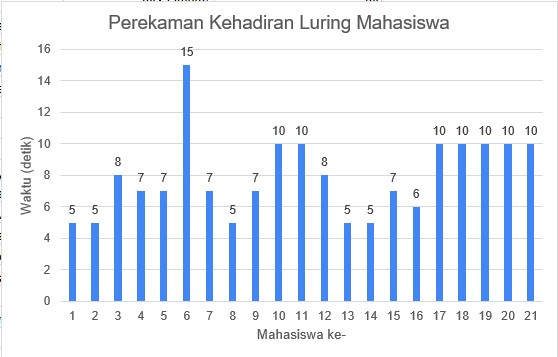
\includegraphics[scale=0.7]{Gambar/LuringMahasiswa.jpg}
		\caption{Histogram Waktu Perekaman Kehadiran Luring Mahasiswa} 
		\label{fig:LuringMahasiswa}
	\end{figure}
	Pada Gambar \ref{fig:LuringMahasiswa} merupakan visualisasi dari hasil survei mengenai lama waktu yang dibutuhkan dari 21 mahasiswa untuk melakukan perekaman kehadiran secara luring. Histogram ini dikelompokan berdasarkan rentang waktu per 20 detik. Histogram tersebut menunjukan bahwa seluruh mahasiswa sebanyak 21 orang memiliki rentang waktu mulai dari 0 sampai 20 detik melakukan perekaman kehadiran secara daring. Hasil survei perekeman kehadiran secara luring untuk setiap mahasiswa secara jelas dapat dilihat pada tabel \ref{tab:luringMahasiswa}. Jawaban dari 21 orang responden adalah mulai dari waktu tercepat 5 detik hingga waktu terlama 15 detik.
	\begin{table}[ht]			
		\caption{Tabel Perekaman Luring Mahasiswa}
		\centering
		\begin{tabular}{|p{4cm} |p{7cm}|}\hline
			Jumlah Responden &  Waktu Perekaman Kehadiran Luring \\ \hline     
			5 orang &  5 detik\\ \hline 
			1 orang &  6 detik\\ \hline 
			5 orang &  7 detik\\ \hline 
			2 orang &  8 detik\\ \hline 
			7 orang &  10 detik\\ \hline 
			1 orang &  15 detik\\ \hline
		\end{tabular}
		\label{tab:luringMahasiswa}
	\end{table}\\ 
	Jika dihitung rata-rata waktu yang dibutuhkan untuk melakukan perekaman kehadiran luring bagi para mahasiswa adalah 7,95 detik. 
\end{enumerate}
Berdasarkan hasil survei terdapat beberapa informasi yang dirasakan mahasiswa ketika dalam melakukan perekaman kehadiran daring. Faktor yang menjadi kendala dalam melakukan perekaman kehadiran daring bagi mahasiswa, sebagai berikut:
\begin{enumerate}
	\item Faktor waktu berpengaruh pada kecepatan dalam melakukan perekaman kehadiran daring. Perkuliahan mahasiswa pada jam-jam padat, seperti jam 7 pagi, 9 pagi, 12 siang, atau 1 siang ini biasanya mahasiswa akan mengalami kendala waktu yang lama untuk dapat melakukan perekaman kehadiran daring.
	\item Faktor internet berpengaruh pada kecepatan dalam perekaman kehadiran daring. Setiap mahasiswa pasti menggunakan internet dari provider yang berbeda sehingga waktu yang dibutuhkan dalam melakukan perekaman kehadiran daring bergantung pada internet yang digunakan oleh mahasiswa.
\end{enumerate}

Kesimpulan dari hasil survei mahasiswa menunjukan bahwa rata-rata waktu yang dibutuhkan secara luring adalah 7,95 detik lebih cepat dibandingkan dengan rata-rata waktu yang dibutuhkan secara daring adalah 63 detik.

\subsubsection{Hasil Survei Dosen} 
Berdasarkan hasil survei yang telah diterima dari 6 orang responden yang merupakan dosen Teknik Informatika Universitas Katolik Parahyangan, dengan pertanyaan yang diajukan kepada responen dan rangkuman jawaban hasil survei sebagai berikut:
\begin{enumerate}
	\item \textbf{Berapa detik perkiraan waktu interaksi yang Anda butuhkan untuk melakukan perekaman kehadiran daring di \url{https://akuhadir.unpar.ac.id} ?}
	
	Pada Gambar \ref{fig:DaringDosen} merupakan visualisasi dari hasil survei mengenai lama waktu yang dibutuhkan dari 6 dosen untuk melakukan perekaman kehadiran secara daring. Histogram ini dikelompokan berdasarkan rentang waktu per 20 detik. Histogram menunjukan bahwa sebanyak 4 dosen memiliki rentang waktu 0 sampai 20 detik, 1 dosen memiliki rentang waktu 21 sampai 40 detik, dan 1 dosen memiliki rentang waktu 101 sampai 120 detik. 
		\begin{figure}[H] \vspace{-0.6cm}
		\centering
		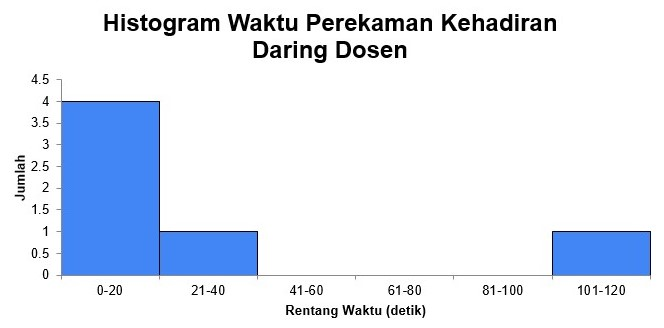
\includegraphics[scale=0.7]{Gambar/DaringDosen.jpg}
		\caption{Histogram Waktu Perekaman Kehadiran Daring Dosen} 
		\label{fig:DaringDosen}
	\end{figure}
	
	Hasil survei perekeman kehadiran daring untuk setiap dosen secara jelas dapat dilihat pada tabel \ref{tab:daringDosen}. Jika dihitung rata-rata waktu yang dibutuhkan untuk melakukan perekaman kehadiran daring bagi para dosen adalah 31,83 detik.
	\begin{table}[ht]			
		\caption{Tabel Perekaman Daring Dosen}
		\centering
		\begin{tabular}{|p{4cm} |p{7cm}|}\hline
			Jumlah Responden &  Waktu Perekaman Kehadiran Daring \\ \hline     
			1 orang &  1 detik\\ \hline 
			1 orang &  10 detik\\ \hline 
			2 orang &  15 detik\\ \hline 
			1 orang &  30 detik\\ \hline 
			1 orang &  120 detik\\ \hline 
		\end{tabular}
		\label{tab:daringDosen}
	\end{table}\\
	\item \textbf{Berapa detik perkiraan waktu interaksi yang Anda butuhkan untuk melakukan perekaman kehadiran luring menggunakan metode fingerprint?}
	
	Pada Gambar \ref{fig:LuringDosen} merupakan visualisasi dari hasil survei mengenai lama waktu yang dibutuhkan dari 6 dosen untuk melakukan perekaman kehadiran secara luring. Histogram ini dikelompokan berdasarkan rentang waktu per 20 detik. Histogram menunjukan bahwa sebanyak 4 dosen memiliki rentang waktu 0 sampai 20 detik, 1 dosen memiliki rentang waktu 21 sampai 40 detik, dan 1 dosen memiliki rentang waktu 81 sampai 100 detik. 
	\begin{figure}[H]
		\centering
		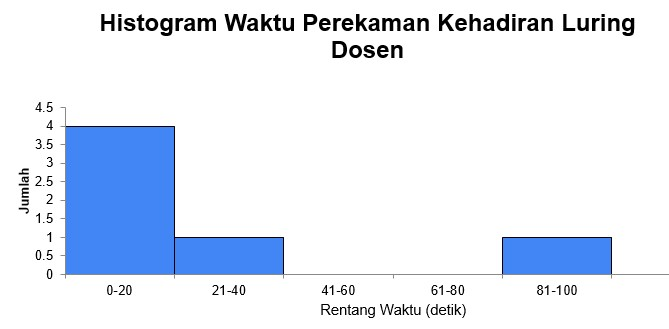
\includegraphics[scale=0.8]{Gambar/LuringDosen.jpg}
		\caption{Histogram Waktu Perekaman Kehadiran Luring Dosen} 
		\label{fig:LuringDosen}
	\end{figure}
	
	Jika dihitung rata-rata waktu yang dibutuhkan untuk melakukan perekaman kehadiran luring bagi para dosen adalah 24,33 detik.Hasil survei perekeman kehadiran luring untuk setiap dosen secara jelas dapat dilihat pada tabel \ref{tab:luringDosen}.	
	\begin{table}[ht]			
		\caption{Tabel Perekaman Luring Dosen}
		\centering
		\begin{tabular}{|p{4cm} |p{7cm}|}
			\hline
			Jumlah Responden &  Waktu Perekaman Kehadiran Luring \\ \hline     
			1 orang &  1 detik\\ \hline 
			3 orang &  5 detik\\ \hline 
			1 orang &  40 detik\\ \hline 
			1 orang &  90 detik\\ \hline 
		\end{tabular}
		\label{tab:luringDosen}
	\end{table}
\end{enumerate}

Kesimpulan dari hasil survei dosen menunjukan bahwa rata-rata waktu yang dibutuhkan secara luring adalah 24,33 detik lebih cepat dibandingkan dengan rata-rata waktu yang dibutuhkan secara daring adalah 31,83 detik.

\subsection{Perekaman Kehadiran Daring ke dalam Selenium}
\label{sec:terjemah} 
Otomatisasi perekaman kehadiran online ini akan menggunakan selenium, sehingga perlu diterjemahkan dari cara perekaman kehadiran online secara normal ke dalam selenium. Membuka situs web \url{https://studentportal.unpar.ac.id/} menggunakan selenium adalah dengan menggunakan \textit{method get()}. Setiap tombol yang ingin ditekan akan diambil elemennya agar dapat diotomatisasikan dengan selenium. Pada \textit{browser} Google Chrome, cara mendapatkan setiap elemen yang dibutuhkan adalah dengan melakukan \textit{inspect} elemen pada bagian yang ingin diambil elemennya. Tombol yang ditekan secara otomatis menggunakan selenium perlu menggunakan \textit{method click()}. Elemen yang ingin diambil dapat dilakukan dengan berbagai macam cara seperti yang sudah dijelaskan pada Bab \ref{sec:selenium}. Beberapa faktor yang dapat dijadikan acuan untuk memilih cara dalam mengambil elemen dapat dilihat dari sebagai berikut:
\begin{enumerate}
	\item Sederhana \\
	Semakin pendek penulisan \textit{query selector} semakin baik dan stabil, misalnya mengambil elemen dengan \textit{CSS selector} yang namanya ``\#username''.
	\item Mudah dimengerti dan dibaca \\
	Menulis \textit{query selector} yang mudah dibaca dan dimengerti sehingga lebih mudah untuk dipahami, contohnya ``\#login-button'' yang artinya memilih elemen tombol untuk \textit{login}. Tidak disarankan menulis \textit{query selector} yang panjang atau sulit dibaca, contohnya mengambil elemen dengan cara XPath seperti yang sudah ditulis pada Bab \ref{sec:selenium} dengan kode program \ref{kode:2:elemenxpath}.
\end{enumerate}
Pemilihan cara pengambilan elemen yang diutamakan adalah dengan mengambil elemen berdasarkan \textit{CSS selector}, tetapi tidak menutup kemungkinan menggunakan cara yang lain untuk menemukan suatu elemen. Jika mengambil elemen berdasarkan \textit{CSS selector} tidak perlu khawatir jika struktur HTML diubah, karena \textit{CSS selector} sangat jarang diubah saat melakukan pembaharuan pada suatu situs web. 
Dalam melakukan otomatisasi perekaman kehadiran online pasti perlu memasukan \textit{email} dan \textit{password}, sehingga untuk memasukan hal tersebut perlu menggunakan \textit{method sendKeys()}. Memasukan \textit{email} dan \textit{password} ini tidak langsung dimasukan ke dalam programnya, tetapi melalui file konfigurasi yang diisi \textit{email} dan \textit{password}, lalu dipanggil ke kode programnya. Program akan berhenti ketika \textit{browser} ditutup atau sudah berhasil melakukan perekaman kehadiran daring secara otomatis.

\subsection{Arsitektur Sistem}
Arsitektur sistem dibuat untuk menjelaskan gambaran umum dari sistem yang akan dibangun. Arsitektur sistem yang dibangun akan menampilkan sebuah program yang dijalankan pada komputer oleh \textit{user}. Diagram arsitektur sistem yang dibangun tampak seperti pada gambar \ref{fig:arsiSistem}.
\begin{figure}[H]
	\centering
	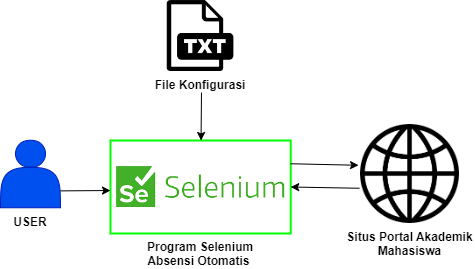
\includegraphics[scale=0.6]{Gambar/arsitekturSistem.png}
	\caption{Diagram Arsitektur} 
	\label{fig:arsiSistem}
\end{figure}
\textit{User} cukup menjalankan program melalui \textit{Command Prompt} pada komputer. Pada sistem ini, program menggunakan \textit{framework} selenium yang berfungsi untuk melakukan otomatisasi pada \textit{browser}. Sistem program ini memiliki sebuah masukan berupa \textit{file} konfigurasi yang berisi perintah-perintah yang akan dijalankan oleh program. Program akan membaca dan menjalankan perintah dari \textit{file} konfigurasi secara baris perbaris. Setiap baris yang dibaca dan dijalankan program akan diteruskan untuk mengotomatisasi \textit{browser} dengan situs Portal Akademik Mahasiswa. Program akan terus membaca dan menjalankan setiap perintah pada \textit{file} konfigurasi hingga akhirnya dapat melakukan perekaman kehadiran secara otomatis pada situs Portal Akademik Mahasiswa. 

\subsection{Pemodelan Diagram \textit{Use Case}}
Salah satu cara untuk mempermudah pembangunan program adalah membuat pemodelan dengan diagram \textit{use case}. Diagram \textit{use case} ini untuk mengetahui interaksi antara pengguna dengan programm. Pemodelan dengan diagram use case ditujukan untuk mempermudah pengembang perangkat lunak dalam memahami kebutuhan fungsional perangkat lunak. Gambar \ref{fig:usecaseUsulan} merupakan diagram use case yang digunakan.

\begin{figure}[H]
	\centering
	\includegraphics[scale=0.6]{Gambar/usecaseUsulan.png}
	\caption{Diagram \textit{Use Case} Sistem Usulan} 
	\label{fig:usecaseUsulan}
\end{figure}

Setelah penggambaran diagram, diperlukan skenario \textit{use case}. Skenario use case ini merupakan alur jalannya proses \textit{use case} dari sisi aktor maupun sisi sistem. Berikut ini merupakan skenario use case yang disajikan dalam bentuk tabel berdasarkan diagram use case sistem usulan pada \ref{fig:usecaseUsulan}.
\begin{enumerate}
	\item \textbf{Skenario mahasiswa melakukan perekaman kehadiran daring otomatis}.
	\begin{itemize}
		\item Nama Use Case: Perekaman kehadiran daring otomatis.
		\item Aktor: Mahasiswa
		\item Deskripsi: Melakukan perekaman kehadiran daring otomatis.
		\item Kondisi awal: -
		\item Kondisi akhir: Program berhasil melakukan perekaman kehadiran secara otomatis.
		\item Skenario utama:
		\begin{table}[h!]
			\centering
			\label{}
			\begin{tabular}{ | m{0.5cm} | m{7cm}| m{6cm} | } 
				\hline
				No & Aksi Aktor & Reaksi Sistem \\ 
				\hline
				1 & Mahasiswa menjalankan program melalui \textit{Command Prompt} dengan direktori \textit{file} & Sistem membuka \textit{browser} Google Chrome.
				\\ 
				\hline
				2 &  & Sistem membuka situs Portal Akademik Mahasiswa dan melakukan \textit{login}.
				\\ 
				\hline
				3 &  & Sistem menuju halaman web perekaman kehadiran daring mahasiswa dan melakukan perekaman kehadiran daring.
				\\ 
				\hline
			\end{tabular}
		\end{table}	
	\end{itemize}
	\item \textbf{Skenario dosen melakukan perekaman kehadiran daring otomatis}.
	\begin{itemize}
		\item Nama Use Case: Perekaman kehadiran daring otomatis.
		\item Aktor: Dosen
		\item Deskripsi: Melakukan perekaman kehadiran daring otomatis.
		\item Kondisi awal: -
		\item Kondisi akhir: Program berhasil melakukan perekaman kehadiran secara otomatis.
		\item Skenario utama:
		\begin{table}[h!]
			\centering
			\label{}
			\begin{tabular}{ | m{0.5cm} | m{7cm}| m{6cm} | } 
				\hline
				No & Aksi Aktor & Reaksi Sistem \\ 
				\hline
				1 & Dosen menjalankan program melalui \textit{Command Prompt} dengan direktori \textit{file} & Sistem membuka \textit{browser} Google Chrome.
				\\ 
				\hline
				2 &  & Sistem membuka situs AKUHADIR dan melakukan \textit{login}.
				\\ 
				\hline
				3 &  & Sistem menuju halaman web perekaman kehadiran daring dosen dan melakukan perekaman kehadiran daring.
				\\ 
				\hline
			\end{tabular}
		\end{table}	
	\end{itemize}
\end{enumerate}
